\section{另一种$L_1$主成分分析}

\begin{frame}{一种最大化特征空间投影$L_1$范数的贪婪算法}
    \begin{itemize}
        \item 交替凸优化算法可以解决问题$P_3$,问题$P_4$也是$L_1$主成分分析。
        \item 回顾$P_4$问题的表述:
    \end{itemize} 
    \small
    \begin{equation}\label{p4}
        P_4: \ \hat{\bm A} = \underset{\bm{A}}{\operatorname{arg \ max}} \| \bm A^T \bm X\|_{L_1}
        = \underset{\bm A}{\operatorname{arg\ max}} 
        \sum_{i=1}^{n}\sum_{k=1}^{m}|\sum_{j=1}^p{a}_{jk}x_{ij}|
         \text{,其中}\bm A^T\bm A = \bm I_m
    \end{equation}
    \begin{itemize}
        \item 当m不为1时,是一个非常复杂的问题。
    \end{itemize} 
\end{frame}

\begin{frame}{一种最大化特征空间投影$L_1$范数的贪婪算法}
    \begin{itemize}
        \item Kwak 于2009年提出一种贪心算法,可以求解该问题。
        \item 首先考虑m为1的情况,在该条件下可以给出一个
        求局部最优解的方法。
    \end{itemize} 
    \begin{figure}
        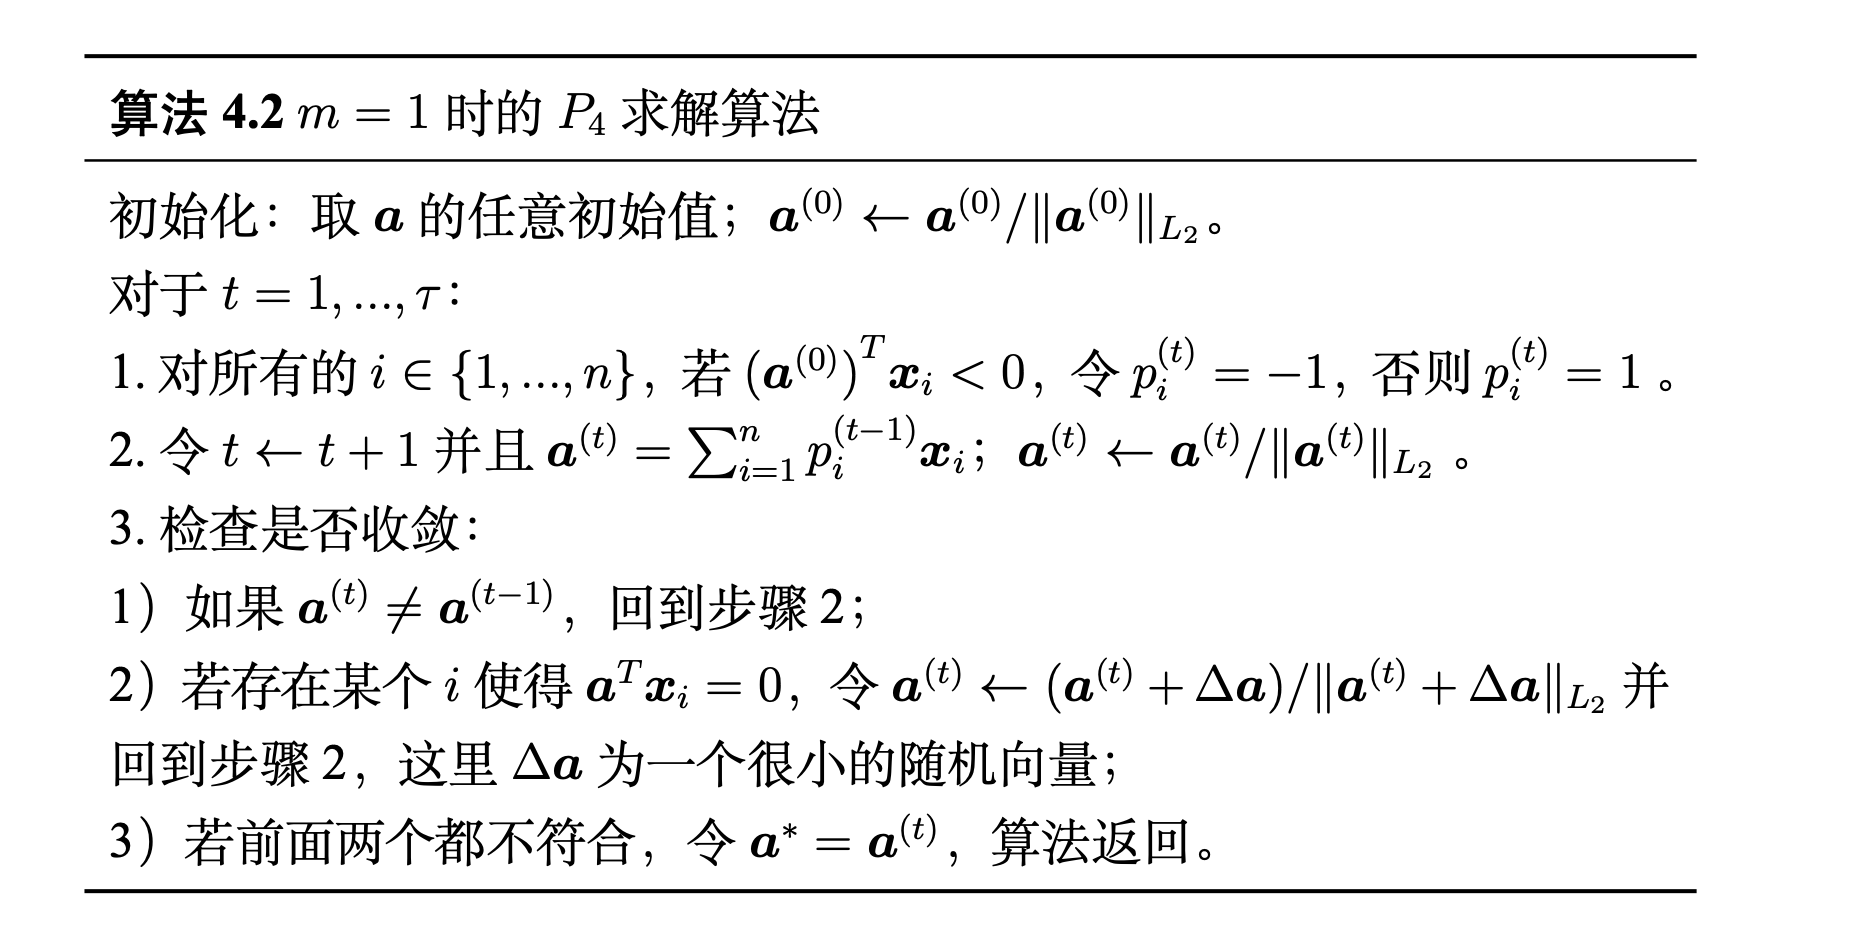
\includegraphics[width=10cm]{pics/kwak-1.png}
    \end{figure}
    \begin{itemize}
        \item 可以证明该算法在有限步骤内收敛到一个局部最优解。
    \end{itemize} 
\end{frame}

\begin{frame}{一种最大化特征空间投影$L_1$范数的贪婪算法}
    \begin{itemize}
        \item 利用贪婪策略,每次求解m为1的子问题,最终得出n个主成分。
    \end{itemize} 
    \begin{figure}
        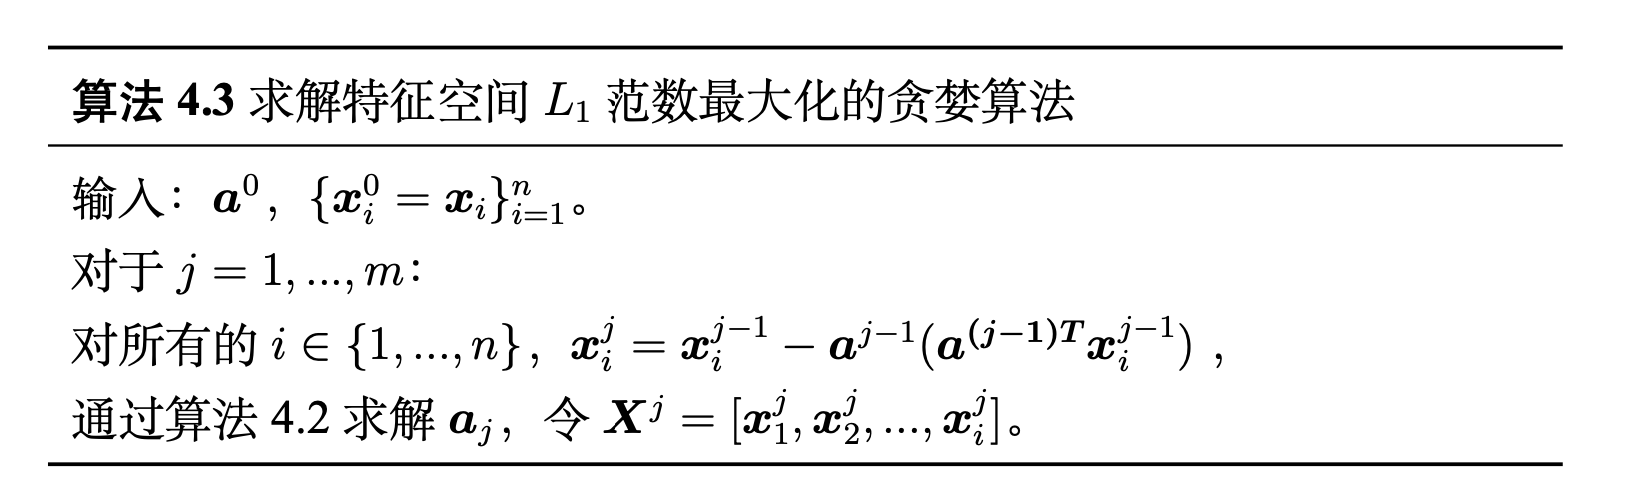
\includegraphics[width=10cm]{pics/kwak-2.png}
    \end{figure}
    \begin{itemize}
        \item 可以证明,算法中每次得到的主成分之间正交。
    \end{itemize} 
\end{frame}


\begin{frame}{数值模拟实验}
    \begin{itemize}
        \item 通过数值模拟实验,希望观察两种$L_1$主成分
        分析和$L_2$主成分析在稳健性和载荷矩阵上的对比。
        \item 可以发现,无论是哪一种$L_1$主成分分析都是
        对离群值稳健的。
    \end{itemize} 
    \begin{figure}
        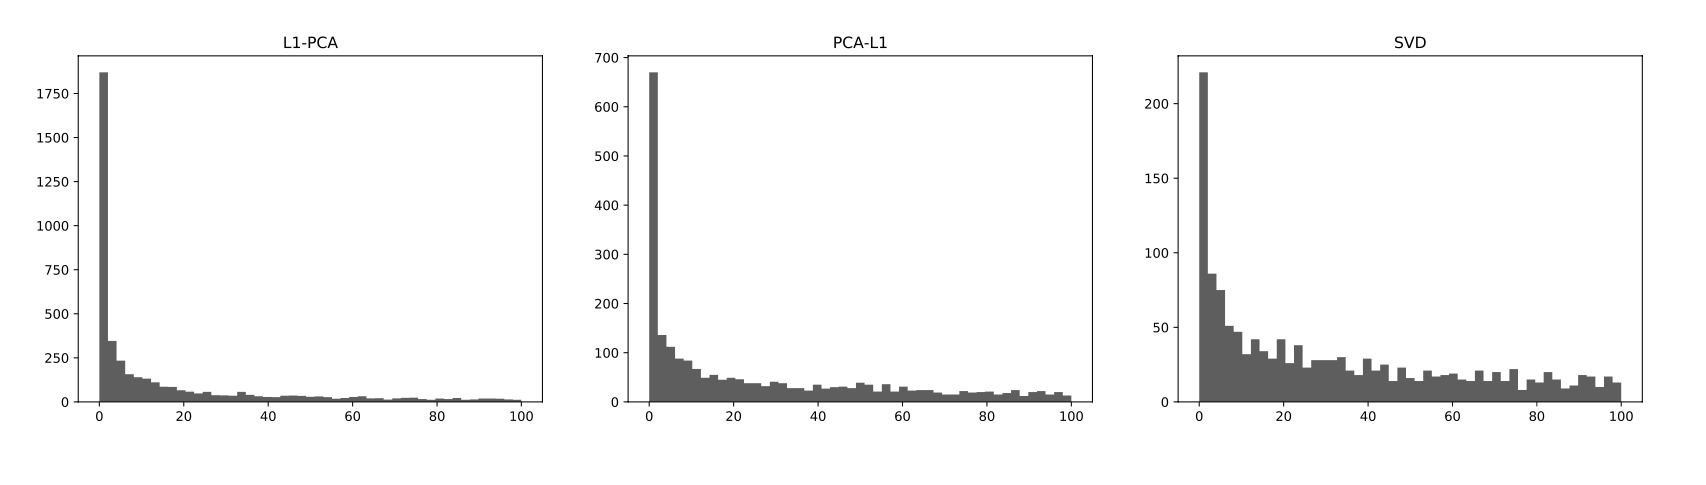
\includegraphics[width=10cm]{pics/compare-l1.png}
    \end{figure}

\end{frame}

\begin{frame}{数值模拟实验}
    \begin{itemize}
        \item 三种主成分分析得到的主成分是不同的。
        \item 将得到的因子载荷矩阵进行最大方差旋转,可更易看出区别。
    \end{itemize} 
    \begin{figure}
        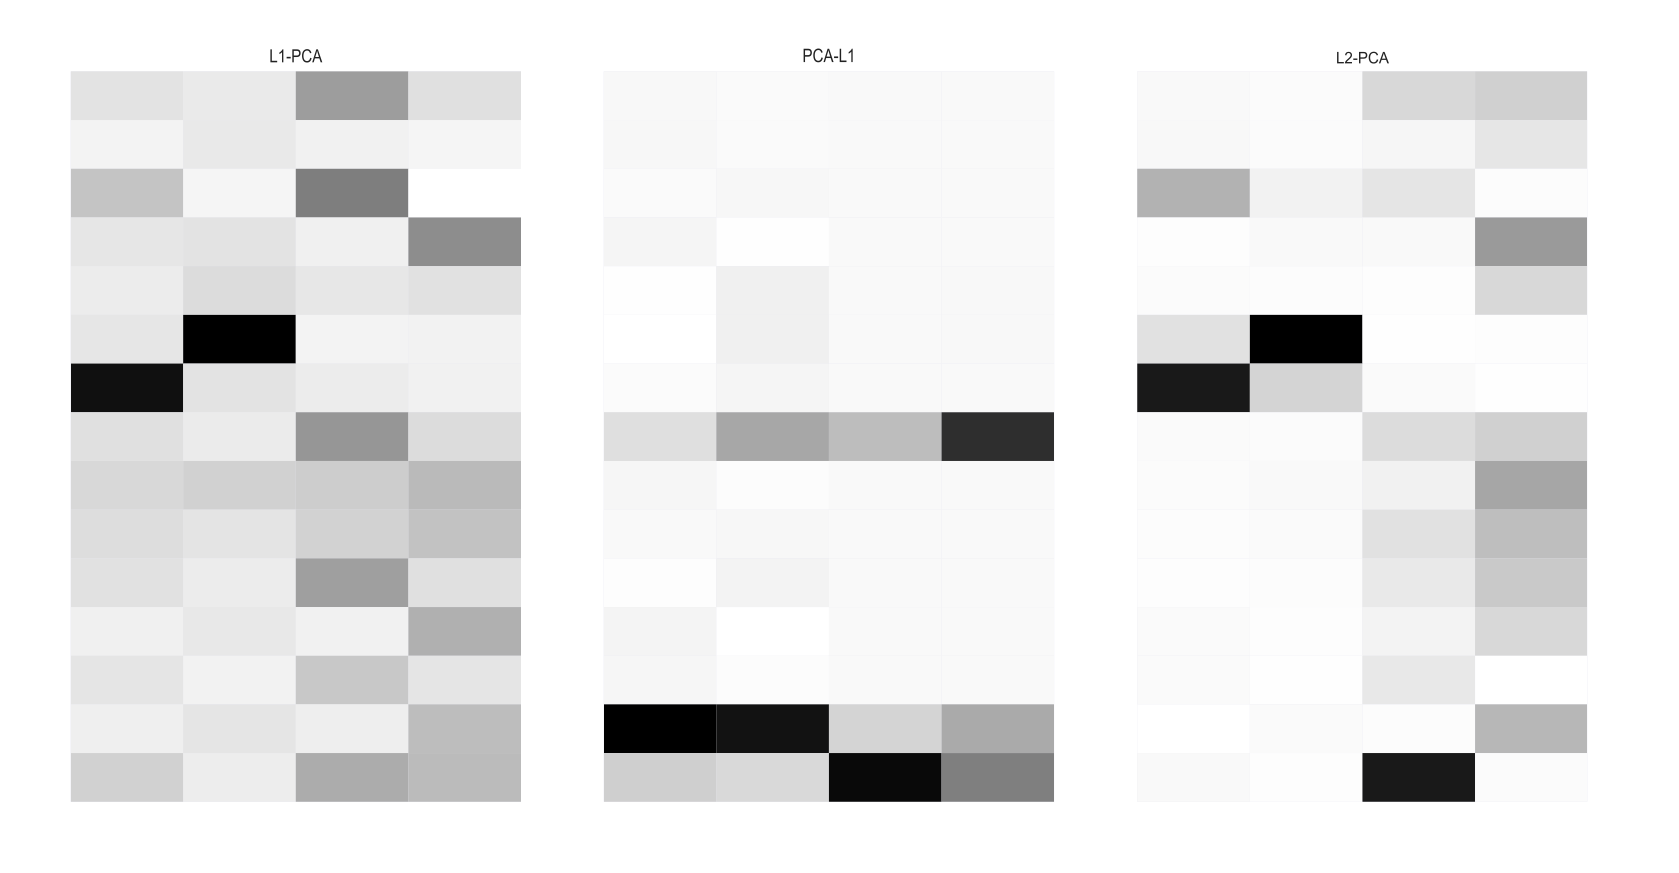
\includegraphics[width=10cm]{pics/loadings-compare.png}
    \end{figure}

\end{frame}


\begin{frame}{实证研究——扩散因子模型进行宏观经济预测}
    \begin{itemize}
        \item 将两种不同的$L_1$主成分分析都应用于扩散指数模型。
        \item 比较预测的准确性,结论是两种$L_1$因子都有良好的
        预测效果,均适用于稳健因子分析。
    \end{itemize} 

    \begin{table}[H]
        \centering
        \tiny
        \caption{向前一个月预测结果}
        \label{outcome4}
        \begin{tabularx}{\textwidth}{lXXXXXX}
        \toprule
                     &  MSE(L1 PCA) &  MSE(PCA L1) &  MAE(L1 PCA) &  MAE(PCA L1) &  MPAE(L1 PCA) &  MPAE(PCA L1) \\ \midrule
        消费者满意指数     & 0.81            & 0.78        & 0.87            & 0.83        & 0.43             & 0.67         \\
        工业生产者出厂价格指数 & 0.70            & 0.83        & 0.75            & 0.92       & 0.96             & 0.90         \\
        货币供应量M2      & 0.76            & 1.01        & 0.90            & 1.00       & 0.45             & 0.92         \\
        固定资产投资总额  & 0.89            & 1.11        & 0.97            & 1.03        & 0.81             & 1.05         \\
        房地产开发投资总额 & 0.79            & 0.94        & 0.95            & 0.97        & 0.91             & 1.10         \\
        社会消费品零售总额 & 0.84            & 0.62        & 0.87            & 0.78        & 0.45             & 0.76         \\
        制造业采购经理指数    & 1.24            & 0.99        & 1.06            & 1.14        & 0.90             & 0.82         \\
        住宅新开工面积总数  & 0.89            & 1.20        & 0.85            & 1.12        & 0.45             & 1.19         \\
        股票流通市值     & 0.99            & 1.23        & 0.98            & 1.12        & 0.81             & 0.98         \\
        消费者信心指数     & 0.93            & 0.70        & 0.98            & 0.80        & 0.98             & 0.99         \\ \bottomrule
        \end{tabularx}
    \end{table}
\end{frame}


\section{结束语}
\begin{frame}{注意}
    \begin{itemize}
        \item 本文所有实验均用Python编程实现了各算法伪代码。
        算法的计算性能与实现程序的质量关联很大,本文的运行时间
        仅做实验对比,不代表算法的标准性能。
    \end{itemize} 
    \small 以SVN算法的一次实现为例给出部分示例代码:
    \begin{figure}
        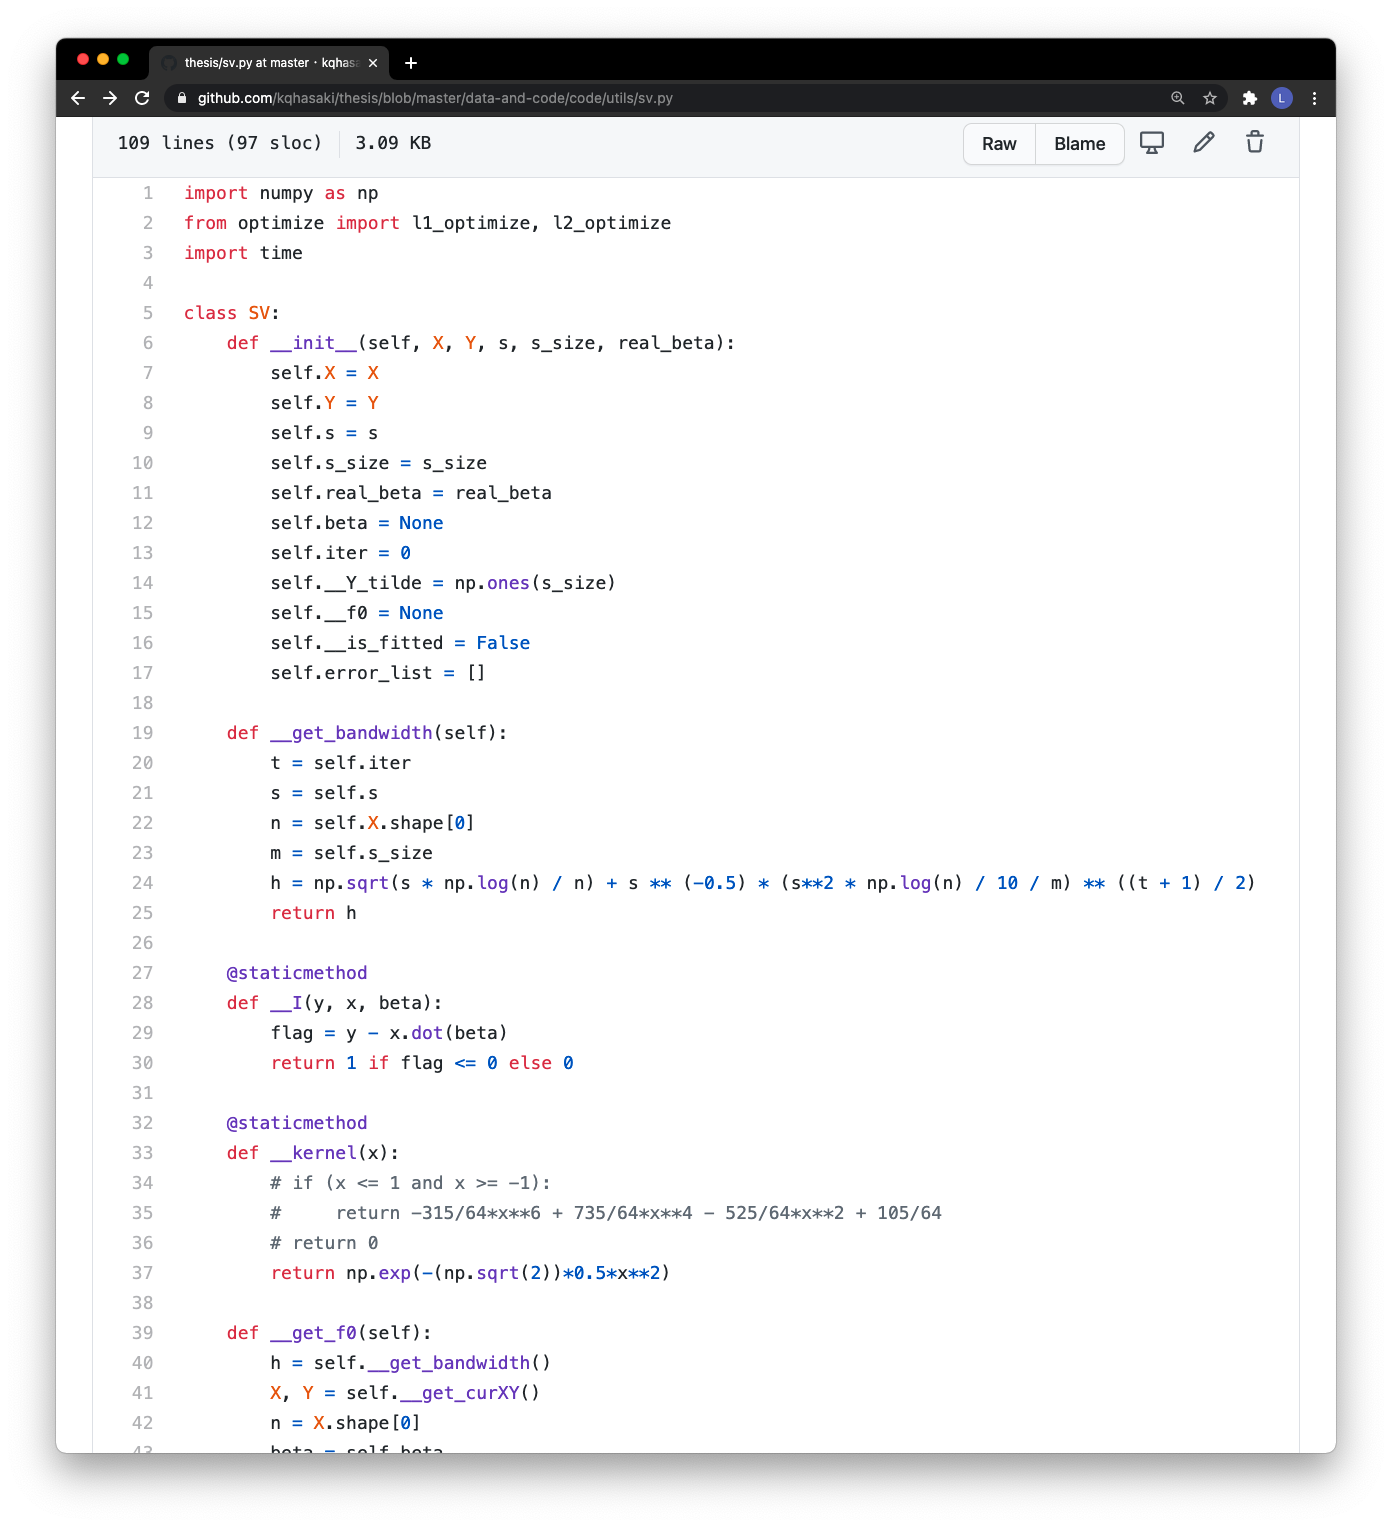
\includegraphics[width=7cm]{pics/code-demo2.png}
    \end{figure}

\end{frame}

\begin{frame}{注意}
    \begin{figure}
        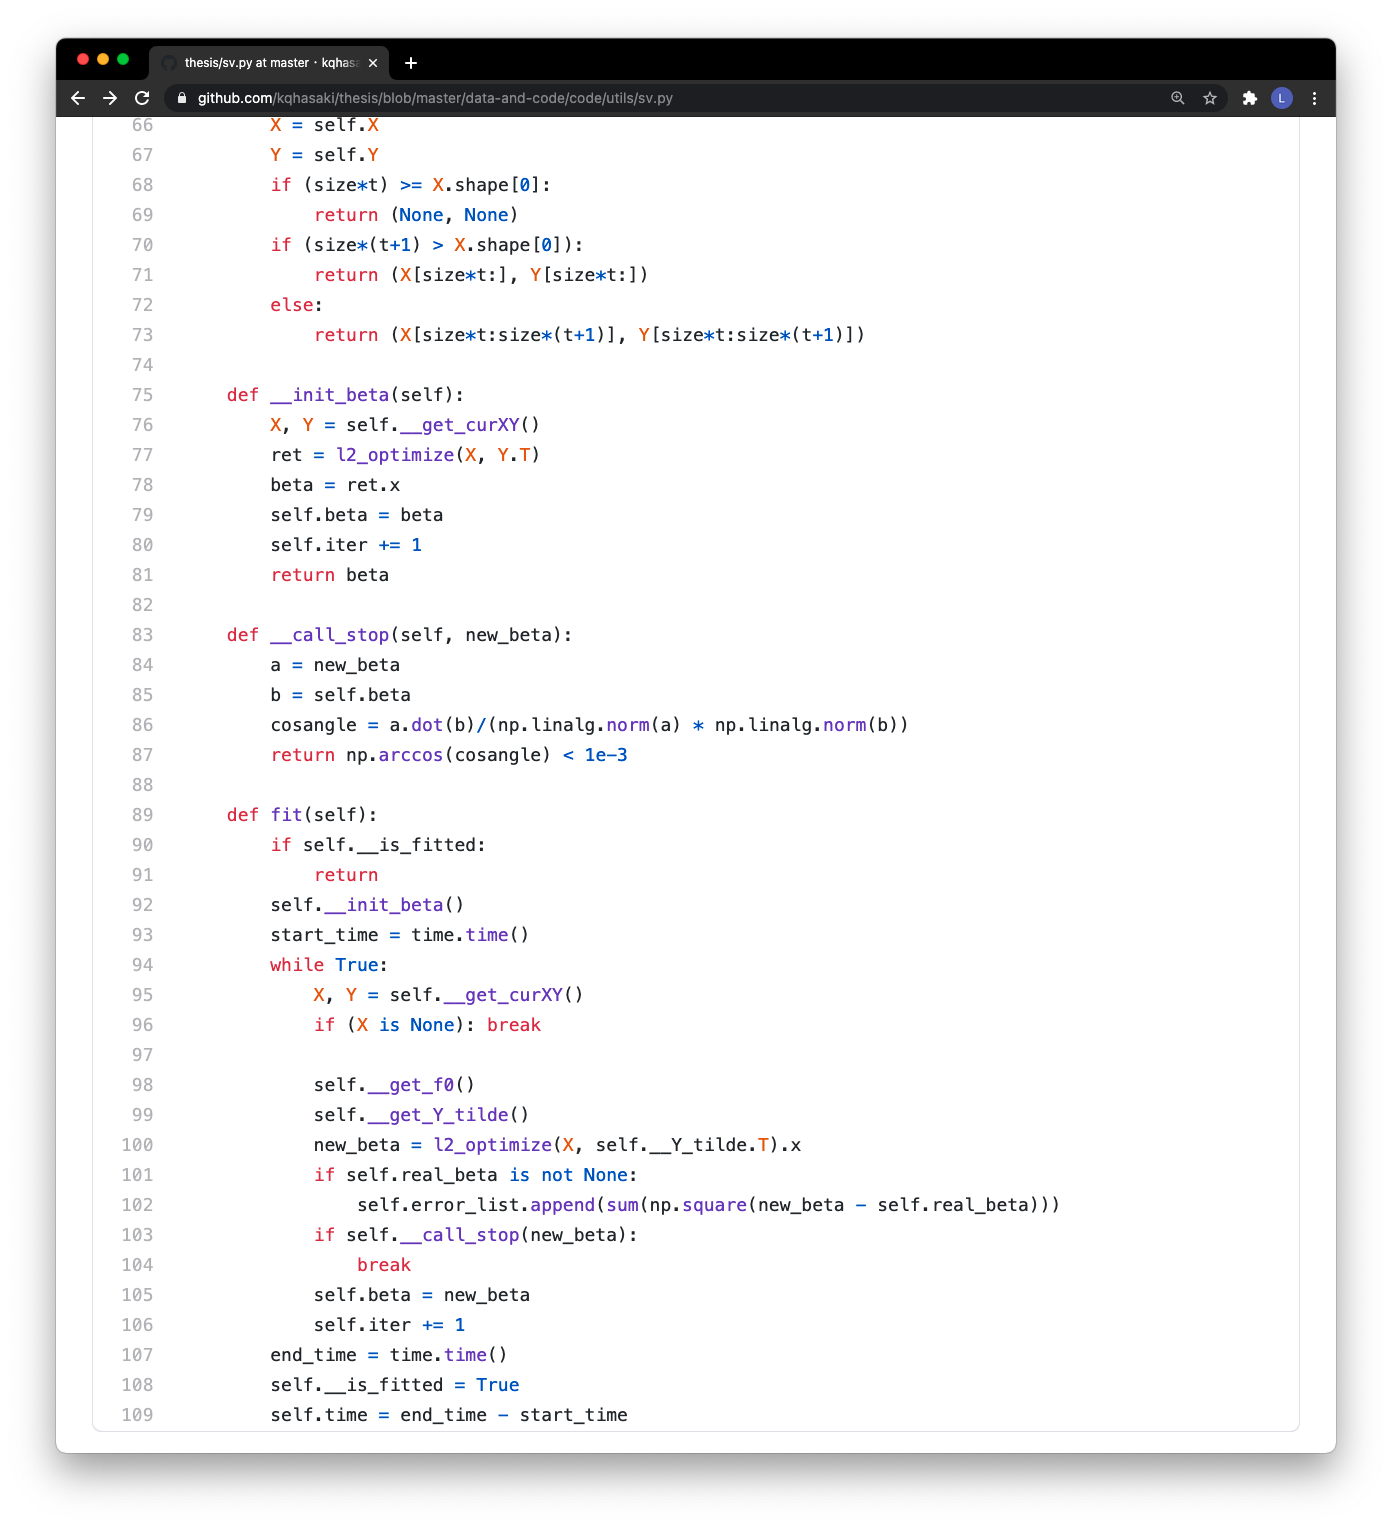
\includegraphics[width=7cm]{pics/code-demo.png}
    \end{figure}
\end{frame}

\begin{frame}{论文的创新点}
    \begin{itemize}
        \item 扩散指数模型进行经济预测时,使用$L_2$主成分估计因子;
        本文创新性地使用$L_1$主成分估计得到$L_1$因子,
        使得在处理重尾宏观经济数据时,预测更加准确、稳健性更好。
        \item 本文介绍并检验了两种最新的最小绝对值回归优化算法,
        并给出了使用建议。
        \item 利用最小绝对值回归优化算法,本文改进了经典的采用
        线性规划的交替凸优化算法,起到了一定的效率改进作用。
    \end{itemize}
\end{frame}



\begin{frame}{结束语}
    \centering
    \Large
    感谢到场的各位专家、教授、老师和同学!
\end{frame}